%-----------------------------------------------------------------------------------------------------------------------------------------------%
%	The MIT License (MIT)
%
%	Copyright (c) 2019 Jan Küster
%
%	Permission is hereby granted, free of charge, to any person obtaining a copy
%	of this software and associated documentation files (the "Software"), to deal
%	in the Software without restriction, including without limitation the rights
%	to use, copy, modify, merge, publish, distribute, sublicense, and/or sell
%	copies of the Software, and to permit persons to whom the Software is
%	furnished to do so, subject to the following conditions:
%	
%	THE SOFTWARE IS PROVIDED "AS IS", WITHOUT WARRANTY OF ANY KIND, EXPRESS OR
%	IMPLIED, INCLUDING BUT NOT LIMITED TO THE WARRANTIES OF MERCHANTABILITY,
%	FITNESS FOR A PARTICULAR PURPOSE AND NONINFRINGEMENT. IN NO EVENT SHALL THE
%	AUTHORS OR COPYRIGHT HOLDERS BE LIABLE FOR ANY CLAIM, DAMAGES OR OTHER
%	LIABILITY, WHETHER IN AN ACTION OF CONTRACT, TORT OR OTHERWISE, ARISING FROM,
%	OUT OF OR IN CONNECTION WITH THE SOFTWARE OR THE USE OR OTHER DEALINGS IN
%	THE SOFTWARE.
%	
%
%-----------------------------------------------------------------------------------------------------------------------------------------------%


%============================================================================%
%
%	DOCUMENT DEFINITION
%
%============================================================================%

%we use article class because we want to fully customize the page and don't use a cv template
\documentclass[10pt,A4]{article}	


%----------------------------------------------------------------------------------------
%	ENCODING
%----------------------------------------------------------------------------------------

% we use utf8 since we want to build from any machine
\usepackage[utf8]{inputenc}		

%----------------------------------------------------------------------------------------
%	LOGIC
%----------------------------------------------------------------------------------------

% provides \isempty test
\usepackage{xstring, xifthen}

%----------------------------------------------------------------------------------------
%	FONT BASICS
%----------------------------------------------------------------------------------------

% some tex-live fonts - choose your own

\usepackage{nth}
%\usepackage[defaultsans]{droidsans}
%\usepackage[default]{comfortaa}
%\usepackage{cmbright}
\usepackage[default]{raleway}
%\usepackage{fetamont}
%\usepackage[default]{gillius}
%\usepackage[light,math]{iwona}
%\usepackage[thin]{roboto} 

% set font default
\renewcommand*\familydefault{\sfdefault} 	
\usepackage[T1]{fontenc}

% more font size definitions
\usepackage{moresize}

%----------------------------------------------------------------------------------------
%	FONT AWESOME ICONS
%---------------------------------------------------------------------------------------- 

% include the fontawesome icon set
\usepackage{fontawesome}

% use to vertically center content
% credits to: http://tex.stackexchange.com/questions/7219/how-to-vertically-center-two-images-next-to-each-other
\newcommand{\vcenteredinclude}[1]{\begingroup
\setbox0=\hbox{\includegraphics{#1}}%
\parbox{\wd0}{\box0}\endgroup}

% use to vertically center content
% credits to: http://tex.stackexchange.com/questions/7219/how-to-vertically-center-two-images-next-to-each-other
\newcommand*{\vcenteredhbox}[1]{\begingroup
\setbox0=\hbox{#1}\parbox{\wd0}{\box0}\endgroup}

% icon shortcut
\newcommand{\icon}[3] { 							
	\makebox(#2, #2){\textcolor{maincol}{\csname fa#1\endcsname}}
}	


% icon with text shortcut
\newcommand{\icontext}[4]{ 						
	\vcenteredhbox{\icon{#1}{#2}{#3}}  \hspace{2pt}  \parbox{0.9\mpwidth}{\textcolor{#4}{#3}}
}

% icon with website url
\newcommand{\iconhref}[5]{ 						
    \vcenteredhbox{\icon{#1}{#2}{#5}}  \hspace{2pt} \href{#4}{\textcolor{#5}{#3}}
}

% icon with openstreetmap url
\newcommand{\iconosm}[4]{
    \iconhref{#1}{#2}{#3}{https://www.openstreetmap.org/search?query=#3}{#4}
}

% icon with email link
\newcommand{\iconemail}[5]{ 						
    \vcenteredhbox{\icon{#1}{#2}{#5}}  \hspace{2pt} \href{mailto:#4}{\textcolor{#5}{#3}}
}

%----------------------------------------------------------------------------------------
%	PAGE LAYOUT  DEFINITIONS
%----------------------------------------------------------------------------------------

% page outer frames (debug-only)
% \usepackage{showframe}		

% we use paracol to display breakable two columns
\usepackage{paracol}

% define page styles using geometry
\usepackage[a4paper]{geometry}

% remove all possible margins
\geometry{top=1cm, bottom=1cm, left=1cm, right=1cm}

\usepackage{fancyhdr}
\pagestyle{empty}

% space between header and content
% \setlength{\headheight}{0pt}

% indentation is zero
\setlength{\parindent}{0mm}

%----------------------------------------------------------------------------------------
%	TABLE /ARRAY DEFINITIONS
%---------------------------------------------------------------------------------------- 

% extended aligning of tabular cells
\usepackage{array}

% custom column right-align with fixed width
% use like p{size} but via x{size}
\newcolumntype{x}[1]{%
>{\raggedleft\hspace{0pt}}p{#1}}%


%----------------------------------------------------------------------------------------
%	GRAPHICS DEFINITIONS
%---------------------------------------------------------------------------------------- 

%for header image
\usepackage{graphicx}

% use this for floating figures
% \usepackage{wrapfig}
% \usepackage{float}
% \floatstyle{boxed} 
% \restylefloat{figure}

%for drawing graphics		
\usepackage{tikz}				
\usetikzlibrary{shapes, backgrounds,mindmap, trees}

%----------------------------------------------------------------------------------------
%	Color DEFINITIONS
%---------------------------------------------------------------------------------------- 
\usepackage{transparent}
\usepackage{color}

% primary color
\definecolor{maincol}{RGB}{ 204, 153, 255 }

% accent color, secondary
% \definecolor{accentcol}{RGB}{ 250, 150, 10 }

% dark color
% \definecolor{darkcol}{RGB}{ 245, 180, 180 }
\definecolor{darkcol}{HTML}{777696}

% light color
\definecolor{lightcol}{RGB}{245,245,245}


% Package for links, must be the last package used
\usepackage[hidelinks]{hyperref}

% returns minipage width minus two times \fboxsep
% to keep padding included in width calculations
% can also be used for other boxes / environments
\newcommand{\mpwidth}{\linewidth-\fboxsep-\fboxsep}
	


%============================================================================%
%
%	CV COMMANDS
%
%============================================================================%

%----------------------------------------------------------------------------------------
%	 CV LIST
%----------------------------------------------------------------------------------------

% renders a standard latex list but abstracts away the environment definition (begin/end)
\newcommand{\cvlist}[1] {
	\begin{itemize}{#1}\end{itemize}
}

%----------------------------------------------------------------------------------------
%	 CV TEXT
%----------------------------------------------------------------------------------------

% base class to wrap any text based stuff here. Renders like a paragraph.
% Allows complex commands to be passed, too.
% param 1: *any
\newcommand{\cvtext}[1] {
	\begin{tabular*}{1\mpwidth}{p{0.98\mpwidth}}
		\parbox{1\mpwidth}{#1}
	\end{tabular*}
}

%----------------------------------------------------------------------------------------
%	CV SECTION
%----------------------------------------------------------------------------------------

% Renders a a CV section headline with a nice underline in main color.
% param 1: section title
\newcommand{\cvsection}[1] {
	\vspace{5pt}
	\cvtext{
		\textbf{\LARGE{\textcolor{darkcol}{\uppercase{#1}}}}\\[-4pt]
		\textcolor{maincol}{ \rule{0.1\textwidth}{2pt} } \\
	}
}

%----------------------------------------------------------------------------------------
%	META SKILL
%----------------------------------------------------------------------------------------

% Renders a progress-bar to indicate a certain skill in percent.
% param 1: name of the skill / tech / etc.
% param 2: level (for example in years)
% param 3: percent, values range from 0 to 1
\newcommand{\cvskill}[3] {
	\begin{tabular*}{1\mpwidth}{p{0.72\mpwidth}  r}
 		\textcolor{black}{\textbf{#1}} & \textcolor{maincol}{#2}\\
	\end{tabular*}%
	
	\hspace{4pt}
	\begin{tikzpicture}[scale=1,rounded corners=2pt,very thin]
		\fill [lightcol] (0,0) rectangle (1\mpwidth, 0.15);
		\fill [maincol] (0,0) rectangle (#3\mpwidth, 0.15);
  	\end{tikzpicture}%
}

%----------------------------------------------------------------------------------------
%	META LANGUAGES
%----------------------------------------------------------------------------------------


% Renders a progress-bar to indicate a certain skill in percent.
% param 1: name of the language
% param 2: level (for example in years)
% param 3: percent, values range from 0 to 1
\newcommand{\cvlanguage}[3] {
	\begin{tabular*}{1\mpwidth}{p{0.72\mpwidth}  r}
 		\textcolor{black}{\textbf{#1}} & \textcolor{maincol}{#2}\\
	\end{tabular*}%
	
	\hspace{4pt}
	\begin{tikzpicture}[scale=1,rounded corners=2pt,very thin]
		\fill [lightcol] (0,0) rectangle (1\mpwidth, 0.15);
		\fill [maincol] (0,0) rectangle (#3\mpwidth, 0.15);
  	\end{tikzpicture}%
}


%----------------------------------------------------------------------------------------
%	 CV EVENT
%----------------------------------------------------------------------------------------

% Renders a table and a paragraph (cvtext) wrapped in a parbox (to ensure minimum content
% is glued together when a pagebreak appears).
% Additional Information can be passed in text or list form (or other environments).
% the work you did
% param 1: time-frame i.e. Sep 14 - Jan 15 etc.
% param 2:	 event name (job position etc.)
% param 3: Customer, Employer, Industry
% param 4: Short description
% param 5: work done (optional)
% param 6: technologies include (optional)
% param 7: achievements (optional)
\newcommand{\cvevent}[7] {
	
	% we wrap this part in a parbox, so title and description are not separated on a pagebreak
	% if you need more control on page breaks, remove the parbox
	\parbox{\mpwidth}{
		\begin{tabular*}{1\mpwidth}{p{0.72\mpwidth}  r}
	 		\textcolor{black}{\textbf{#2}} & \colorbox{maincol}{\makebox[0.25\mpwidth]{\textcolor{white}{#1}}} \\
			\textcolor{maincol}{\textbf{#3}} & \\
		\end{tabular*}\\[8pt]
	
		\ifthenelse{\isempty{#4}}{}{
			\cvtext{#4}\\
		}
	}

	\ifthenelse{\isempty{#5}}{}{
		\vspace{9pt}
		{#5}
	}

	\ifthenelse{\isempty{#6}}{}{
		\vspace{9pt}
		\cvtext{\textbf{Technologies include:}}\\
		{#6}
	}

	\ifthenelse{\isempty{#7}}{}{
		\vspace{9pt}
		\cvtext{\textbf{Achievements include:}}\\
		{#7}
	}
	\vspace{10pt}
	\vspace{10pt}
    \vspace{-0.5cm}
}

%----------------------------------------------------------------------------------------
%	 CV META EVENT
%----------------------------------------------------------------------------------------

% Renders a CV event on the sidebar
% param 1: title
% param 2: subtitle (optional)
% param 3: customer, employer, etc,. (optional)
% param 4: info text (optional)
\newcommand{\cvmetaevent}[4] {
	\textcolor{maincol} {\cvtext{\textbf{\begin{flushleft}#1\end{flushleft}}}}

	\ifthenelse{\isempty{#2}}{}{
	\textcolor{darkcol} {\cvtext{\textbf{#2}} }
	}

	\ifthenelse{\isempty{#3}}{}{
		\cvtext{{ \textcolor{darkcol} {#3} }}\\
	}

	\ifthenelse{\isempty{#4}}{}{
	    \cvtext{#4}\\[2pt]
    }
    \vspace{-0.5cm}
}

%---------------------------------------------------------------------------------------
%	QR CODE
%----------------------------------------------------------------------------------------

% Renders a qrcode image (centered, relative to the parentwidth)
% param 1: percent width, from 0 to 1
\newcommand{\cvqrcode} {
	\begin{center}
		
\includegraphics[width=0.7\mpwidth]{../resources/imgs/qrcode.png}
	\end{center}
}


\newcommand{\makecolorbox}[1]{
    \colorbox{maincol}{\makebox[0.25\mpwidth]{\textcolor{white}{#1}}}
}


%============================================================================%
%
%
%
%	DOCUMENT CONTENT
%
%
%
%============================================================================%
\begin{document}
% \columnratio{0.3}
\columnratio{0.27}
\setlength{\columnsep}{2.2em}
\setlength{\columnseprule}{4pt}
\colseprulecolor{lightcol}
\begin{paracol}{2}
\begin{leftcolumn}
%---------------------------------------------------------------------------------------
%	META IMAGE
%----------------------------------------------------------------------------------------
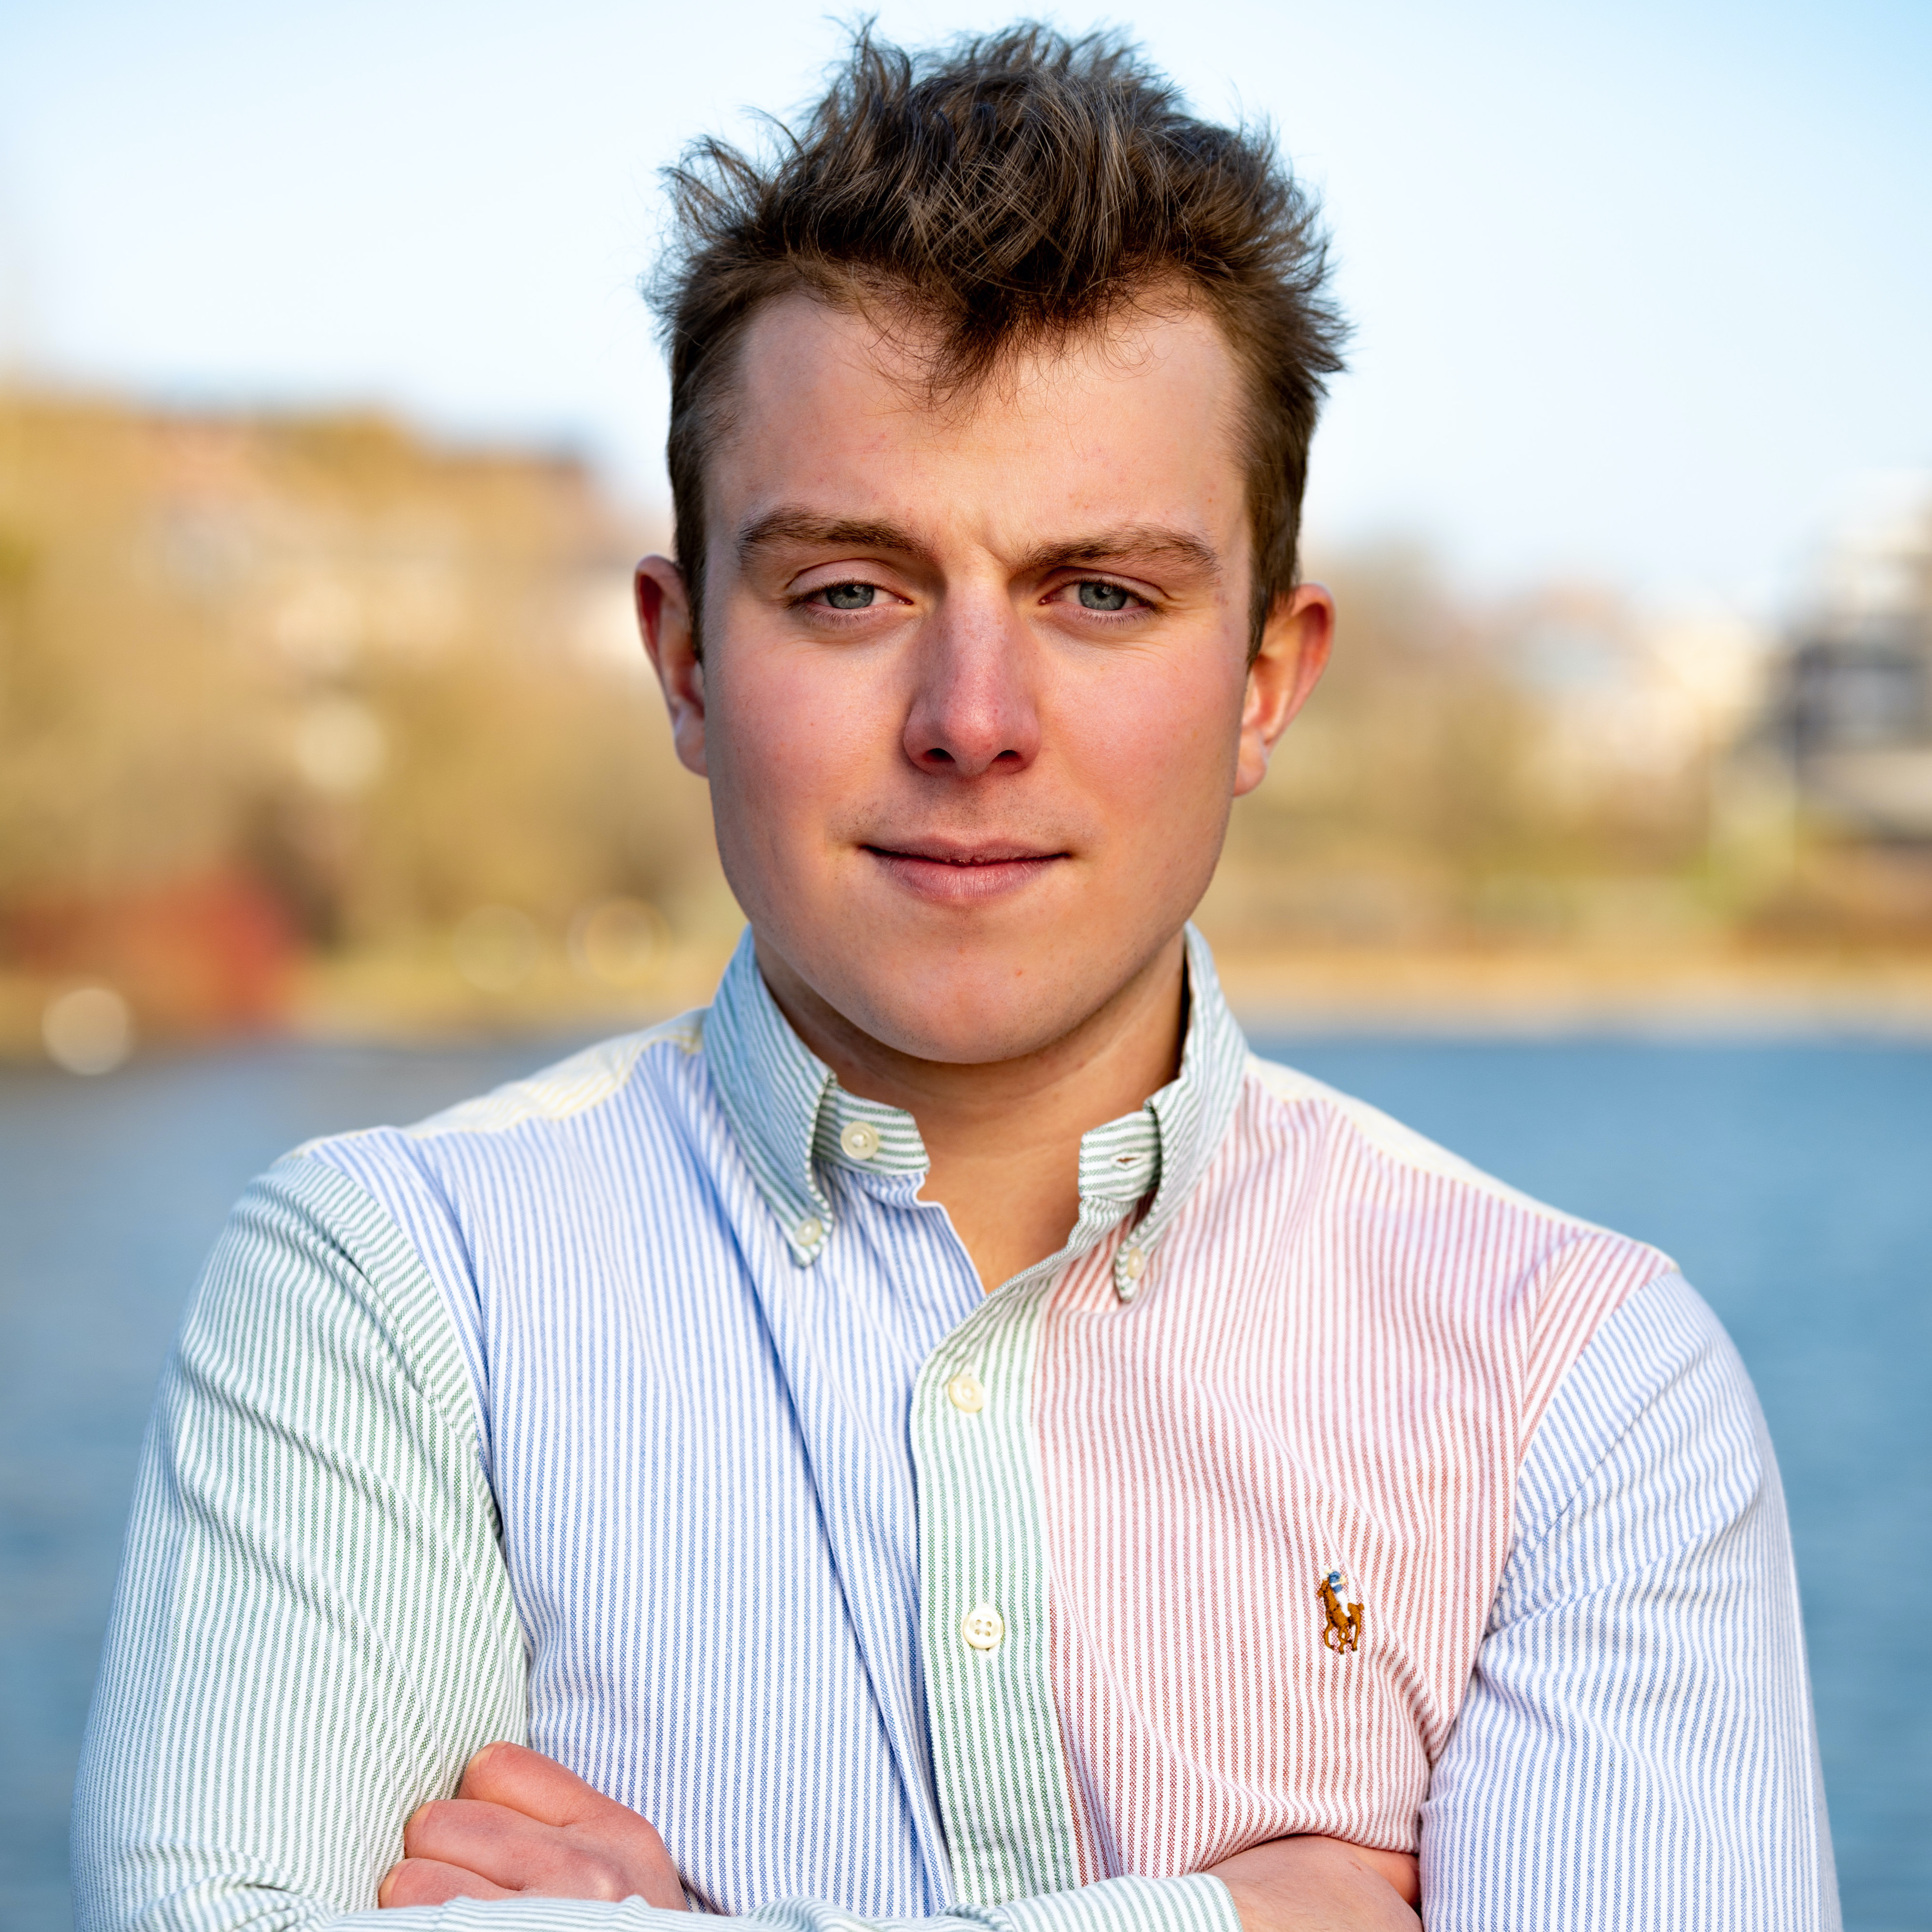
\includegraphics[width=\linewidth]{../resources/imgs/profile1.png}	%trimming relative to image size

%---------------------------------------------------------------------------------------
%	META SKILLS
%----------------------------------------------------------------------------------------
\cvsection{PERSONAL}
	
\iconhref{BirthdayCake}{12}{14th August 1999}{}{black}\\[6pt]
% \iconhref{MapMarker}{12}{Buisson Ponsin 10,\\ 6800 Libramont-Chevigny,\\ Belgium}{https://www.openstreetmap.org/way/945440098\#map=18/49.90597/5.40513}{black}\\[6pt]
\iconhref{MapMarker}{12}{Route Neuve 3,\\1024 Ecublens (VD),\\Switzerland}{https://www.openstreetmap.org/way/283233106\#map=19/46.52887/6.56117}{black}\\[6pt]
\iconhref{MobilePhone}{12}{+41 78 231 14 77}{tel:+41782311477}{black}\\[6pt]
% \iconemail{Envelope}{12}{graux.romain@protonmail.com}{graux.romain@protonmail.com}{black}\\[6pt]
\iconemail{Envelope}{12}{romaingrx@duck.com}{romaingrx@duck.com}{black}\\[6pt]

\cvsection{LANGUAGES}

\cvlanguage{French} {Native} {1.0} \\[-2pt]
\cvlanguage{English} {Fluent} {0.9} \\[-2pt]


% \vfill\null
\cvsection{LINKS}

\iconhref{Github}{12}{RomainGrx}{https://github.com/RomainGrx}{black}\\[6pt]
\iconhref{Linkedin}{12}{romaingraux}{https://www.linkedin.com/in/romaingraux/}{black}\\[6pt]

% \vfill\null
\cvsection{LICENSES}

\iconhref{Car}{12}{B, BE}{}{black}\\[6pt]
\iconhref{Anchor}{12}{ICC (inland and coast, motor and sail)}{}{black}\\[6pt]


%---------------------------------------------------------------------------------------
%	CERTIFICATION
%----------------------------------------------------------------------------------------
\cvsection{CERTIFICATIONS}

\cvmetaevent
{Jul 2020 - Jul 2023}
{\href{https://www.credential.net/326a136c-9842-42ba-a96d-0786c3dba813}{TensorFlow Developer Certificate}}
{}
{}

\vspace{10pt}
\vfill\null
\cvqrcode{}

% \vfill\null
% \cvsection{SKILLS}
% 
% \cvskill{Python} {4+ yrs} {0.95} \\[-2pt]
% \cvskill{C/C++} {3+ yrs} {0.7} \\[-2pt]
% \cvskill{Java} {3+ yrs} {0.7} \\[-2pt]
% \cvskill{Linux} {3+ yrs} {0.6} \\[-2pt]
% \cvskill{GIT} {3+ yrs} {0.6} \\[-2pt]
% \cvskill{Vim} {2+ yrs} {0.6} \\[-2pt]
% \cvskill{Go} {1+ yrs} {0.5} \\[-2pt]
% \begin{center}
%     \vspace{-1em}
%     \tiny{non-exhaustive list...}
% \end{center}



% \newpage
% \mbox{} % hotfix to place qrcode on the bottom when there are not other elements
% \vfill
% \cvqrcode{}

\end{leftcolumn}
\begin{rightcolumn}
%---------------------------------------------------------------------------------------
%	TITLE  HEADER
%----------------------------------------------------------------------------------------
\fcolorbox{white}{darkcol}{\begin{minipage}[c][3.5cm][c]{1\mpwidth}
	\begin {center}
		\HUGE{ \textbf{ \textcolor{white}{ \uppercase{ROMAIN GRAUX} } } } \\[-24pt]
		\textcolor{white}{ \rule{0.1\textwidth}{1.25pt} } \\[4pt]
		\large{ \textcolor{white} {Data Science/Cryptography student} }
	\end {center}
\end{minipage}} \\[14pt]
\vspace{-12pt}

%---------------------------------------------------------------------------------------
%	PROFILE
%----------------------------------------------------------------------------------------
% \vfill\null
% \cvsection{PROFILE}
% 
% \cvtext{
%     % Facts
%     I'm a young student of $22$ years old in last year of master in Data Science at EPFL. Initially made in Belgium, I moved to Switzerland in September $2021$ in order to finish my master and explore the landscapes.
% 
% 
%     \vspace{1em}
%     % Interests
%     I am really interested in many topics such as cybersecurity, artificial intelligence or even computer network. 
%     But this is not an exhaustive list, I am always hungry to learn and be challenged on any topics (even topics far from bits and electricity).
% 
%     \vspace{1em}
%     % Free time
%     During my free time I usually do bike (trial and downhill), water sport (Boat, wakeboard, ski, \dots) or any sport that keeps me in shape (tennis, rowing, swimming, \dots).
% 
%     }

%---------------------------------------------------------------------------------------
%	EDUCATION
%----------------------------------------------------------------------------------------
\cvsection{EDUCATION}

\cvmetaevent
{2021 - 2022}
{M.S. Data Science Engineering}
{\href{https://www.epfl.ch}{École Polytechnique Fédérale de Lausanne}}
{}

\cvmetaevent
{2020 - 2022}
{M.S. Data Science Engineering}
{\href{https://uclouvain.be/en/faculties/epl}{École Polytechnique de Louvain}}
{}

\cvmetaevent
{2017 - 2020}
{B. Sc. Engineering}
{\href{https://uclouvain.be/en/faculties/epl}{École Polytechnique de Louvain}}
{}

\cvmetaevent
{2011 - 2017}
{High School Degree}
{Institut Saint-Joseph}
{}

%---------------------------------------------------------------------------------------
%	WORK EXPERIENCE
%----------------------------------------------------------------------------------------
\vfill\null
\cvsection{EXPERIENCE}

\cvevent
    {Sep 19 - Sep 21}
    {IT \& Knowledge Manager}
    {\href{https://afdimpact.org/}{Academics For Development}}
    {In charge of the website development of \href{https://afdimpact.org/}{Academics For Development} and all the team accounts and access. Academics for Development is a non-profit organization founded on social entrepreneurship. Through projects and on-campus events, we strive to give students the opportunity to enrich themselves and have durable social impact.}
    {}
    {}
    {}

\cvevent 
 	{Sep 20 - Jun 21}
    {Teaching Assistant}
    {\href{https://uclouvain.be/en/faculties/epl}{École Polytechnique de Louvain}}
    {
        I gave practice sessions to students (between 20 and 50 per session) for 5 different courses (Algorithmique et structures de données, Mathématiques discrètes et probabilité, Méthodes numériques, Signaux et Sytèmes, Informatique 1/Python).
        % \cvlist{
        % \item \makecolorbox{LINFO1121} \href{https://sites.uclouvain.be/archives-portail/cdc2020/en-cours-2020-linfo1121}{Algorithmique et structures de données}
        % \item \makecolorbox{LEPL1108} \href{https://sites.uclouvain.be/archives-portail/cdc2020/en-cours-2020-lepl1108}{Mathématiques discrètes et probabilité}
        % \item \makecolorbox{LEPL1104} \href{https://sites.uclouvain.be/archives-portail/cdc2020/en-cours-2020-lepl1104}{Méthodes numériques}
        % \item \makecolorbox{LEPL1106} \href{https://sites.uclouvain.be/archives-portail/cdc2020/en-cours-2020-lepl1106}{Signaux et Sytèmes}
        % \item \makecolorbox{LEPL1401} \href{https://sites.uclouvain.be/archives-portail/cdc2020/en-cours-2020-lepl1401}{Informatique 1}
        % }
    }   
	{}
	{}
	{}

\cvevent
	{Aug 20 - Sep 20}
	{Computer Vision Internship}
	{\href{https://www.aerospacelab.be/}{Aeorspacelab}}
    {Joined a team of machine learning engineers for one month internship at \href{https://www.aerospacelab.be/}{Aeorspacelab} building Computer Vision models, data cleaning and web scraping concerning satellite images and location informations.}
	{}
	{}
	{}

% \cvevent
% 	{Aug 19 - Sep 19}
% 	{Automative Expertise Trainee}
% 	{\href{https://experts-partners.org}{Experts Partners}}
%     {
%     Working with an automotive Senior Expert in the field and records encoding back in the office.
%     }
% 	{}
% 	{}
% 	{}

\cvevent 
 	{Sep 18 - Aug 19}
    {Project Student}
    {\href{https://afdimpact.org}{Academics For Development}}
    {
        Fundraising, design and building of a water pump powered by solar energy in a village (Edouwossikopé) in Togo.
         More information about the project : \url{https://afdimpact.org/projectname/p\_lln\_1819\_odeah\_togo/}
    }   
	{}
	{}
	{}

% hotfixes to create fake-space to ensure the whole height is used
\mbox{}
\vfill
\mbox{}
\vfill
\mbox{}
\vfill
\mbox{}
\end{rightcolumn}
\end{paracol}
\end{document}
